\begin{proofbox}
\textbf{\textcolor{CProof}{证明目标}}\par
证明“$(m,n)$内恰有两个\textbf{不同}零点”与
$\Delta>0,\ m<x_0<n,\ af(m)>0,\ af(n)>0$\textbf{互相推出}。三种方法从图像到代数，由浅入深。

\medskip
\textbf{\textcolor{CProof}{方法一｜画图法（最容易理解）}}\par
\textbf{从根推条件：}两次穿过$x$轴，故$\Delta>0$；对称轴在两交点中间，必须在$(m,n)$内；两端在交点的外侧，所以端点函数值与$a$同号。
\par\textbf{从条件推根：}$\Delta>0$先保证有两个不同交点；对称轴在区间内说明交点分居其左右；$af(m)>0$确保左端点在左交点左侧（不可能在两交点之间）；右端同理。于是两根都在区间内。
\begin{center}
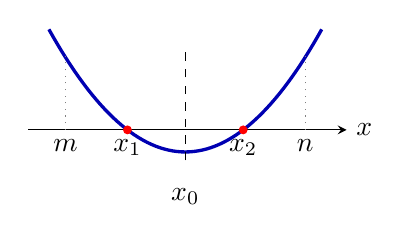
\begin{tikzpicture}[x=1.05cm,y=.88cm,>=stealth]
 \draw[->] (-1.9,0)--(1.95,0) node[right]{$x$};\draw[very thick,blue!70!black,domain=-1.65:1.65,samples=65] plot (\x,{.65*(\x*\x-.49)});
 \draw[dashed] (0,-.44)--(0,1.22);\draw[dotted,gray] (-1.45,0)--(-1.45,1.1) (1.45,0)--(1.45,1.1);
 \node[below] at (-1.45,0) {$m$};\node[below] at (-.7,0) {$x_1$};\node[below] at (0,-.7) {$x_0$};\node[below] at (.7,0) {$x_2$};\node[below] at (1.45,0) {$n$};
 \fill[red] (-.7,0) circle(1.6pt) (.7,0) circle(1.6pt);
\end{tikzpicture}

\end{center}

\medskip
\textbf{\textcolor{CProof}{方法二｜两根的中点法（步骤最少）}}\par
设两根$x_1<x_2$，它们的中点是$x_0=(x_1+x_2)/2$。当$\Delta>0$时已知$x_1<x_0<x_2$。
\par\textbf{左边：}因为$m<x_0$且$af(m)>0$，$m$不能位于$(x_1,x_2)$内，也不能在两根上，只可能$m<x_1$。\textbf{右边：}因为$x_0<n$且$af(n)>0$，同理$x_2<n$。合起来就是$m<x_1<x_2<n$。
\par 反过来若$m<x_1<x_2<n$，其中点当然在区间内，两个端点也都在两根外侧，四个条件自然成立。
\begin{center}
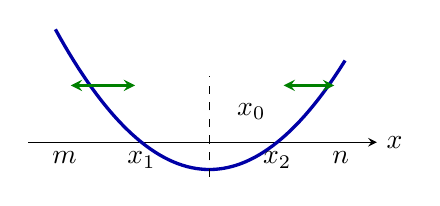
\begin{tikzpicture}[x=1.15cm,y=.88cm,>=stealth]
 \draw[->] (-1.9,0)--(1.95,0) node[right]{$x$};
 \draw[very thick,blue!65!black,domain=-1.6:1.6,samples=65] plot (\x,{.7*(\x+.65)*(\x-.85)});
 \draw[dashed] (.1,-.5)--(.1,.95);
 \node[below] at (-1.5,0) {$m$};\node[below] at (-.65,0) {$x_1$};\node[above right] at (.3,.18) {$x_0$};\node[below] at (.85,0) {$x_2$};\node[below] at (1.55,0) {$n$};
 \draw[<->,green!50!black,thick] (-1.43,.82)--(-.72,.82);
 \draw[<->,green!50!black,thick] (.92,.82)--(1.48,.82);
\end{tikzpicture}

\end{center}

\medskip
\textbf{\textcolor{CProof}{方法三｜因式分解法（常规严格证明）}}\par
$\Delta>0$时，可写成$f(x)=a(x-x_1)(x-x_2)$，其中$x_1<x_2$。于是
\[af(t)=a^2(t-x_1)(t-x_2),\qquad a^2>0.\]
因此$af(t)>0$恰好说明$t<x_1$或$t>x_2$。
\par 又$m<x_0<x_2$，所以$af(m)>0$不可能对应$m>x_2$，只能$m<x_1$；同理$x_1<x_0<n$，$af(n)>0$只能对应$n>x_2$。得$m<x_1<x_2<n$。反向代入因式分解式即可证得全部条件。
\begin{center}
\begin{tikzpicture}[x=1.04cm,y=.9cm,>=stealth]
 \draw[->] (-1.85,0)--(1.9,0) node[right]{$x$};
 \draw[very thick,orange!75!black,domain=-1.6:1.6,samples=65] plot (\x,{-.64*(\x*\x-.64)});
 \node[below] at (-1.5,0) {$m$};\node[below] at (-.8,0) {$x_1$};\node[below] at (0,0) {$x_0$};\node[below] at (.8,0) {$x_2$};\node[below] at (1.5,0) {$n$};
 \node[below] at (0,-1.8) {$a<0$时同样成立};
 \fill[green!50!black] (-1.5,{-.64*(1.5*1.5-.64)}) circle(1.6pt) (1.5,{-.64*(1.5*1.5-.64)}) circle(1.6pt);
\end{tikzpicture}

\end{center}

\medskip
\textbf{\textcolor{CProof}{补证｜“恰一个零点”为什么要分情况？}}\par
\textbf{两端异号时：}若$\Delta<0$没有根、$\Delta=0$只在顶点碰到轴，均不会让两端异号；所以有两个不同实根。将两根从左到右排好后，函数符号每经过一个不同根改变一次。端点符号相反，说明两端之间恰跨过\textbf{一个}不同的根（不可能跨过两个）。
\par\textbf{重根时：}$\Delta=0$且$m<x_0<n$，$f(x)=a(x-x_0)^2$，仅在$x_0$取零，尽管$f(m)f(n)>0$。
\par\textbf{端点为根时：}$\Delta>0$，设$x_1<x_2$，要么左根不在区间而右根在内（$x_1\le m<x_2<n$），要么左根在内而右根不在内（$m<x_1<n\le x_2$）。这也是结论一给出的完整逐根判定。图中右根就在$n$上，\textbf{不算区间内的根}。
\begin{center}
\begin{tikzpicture}[x=1.08cm,y=.9cm,>=stealth]
 \draw[->] (-1.45,0)--(1.65,0) node[right]{$x$};
 \draw[very thick,blue!75!black,domain=-1.1:1.4,samples=65] plot (\x,{.7*(\x+.45)*(\x-1.0)});
 \node[below] at (-1.15,0) {$m$};\node[below] at (-.45,0) {$x_1$};\node[below right] at (1,-.4) {$n=x_2$};
 \fill[red] (-.45,0) circle(1.7pt);\draw[red,fill=white,thick] (1,0) circle(2.2pt);
 \node[above] at (.1,.9) {内部只数到一个};
\end{tikzpicture}

\end{center}
\textbf{\textcolor{CProof}{结论：}}两根的条件是完整的充要条件；\textbf{两端异号只是单根问题的一种情形}，重根和端点根不能漏。
\end{proofbox}
